%% • The introduction must be dynamite. 
%% – The reader forms an oppinion of the work right from the start... 
%% • The introduction is an extension of the abstract. 
%% • Should be easy to read and understand 
%% • Should make it easy for anyone to tell
%% – What your paper is about 
%%   – What problem it solves
%%   – Why the problem and solution is interesting and relevant (motivation and context). Is it a long- outstanding problem?
%%   – What is new in your paper and how (much) does it improve on the strongest alternatives/previous work (include a few of the most relevant references here).

%% • Start the introduction with the motivation. Think in large contexts and don’t be afraid to be a poet.
%% • All implications, contributions and keypoints of your work must be included here.
%% • Make it very clear how your work will impact the future of Realistic image generation (will people use it?).
%% • If your work is pioneering, s-p-e-l-l i-t o-u-t.
%% • Briefly make it clear how you evaluate your method in the Results section.
%% • Make sure to explain where your method applies and where it does not apply (limitations).


\chapter{Introduction}

\chapterquote{Focus is a matter of deciding what things you're not
  going to do.}{John Carmack}


% Motivation

\textit{Rendering} is the process of converting a scene description into an
image and lies at the heart of \textit{computer graphics}. The ability to render
complex scenes realistically or distinctly is vital in several areas; computer
games, movies and even medical imaging. A scene is made up of models, which can
consist of several thousand geometric primitives, usually triangles. \fixme{Kan
  dette gøres mere læsevenligt?}Information about these triangles are stored at
the vertices and can be its position, a normal perpendicular to its surface or
its color among other things. Such information stored at a triangle's vertices
are called \textit{vertex attributes}.


% Rasterization and cube mapping

When real-time rendering is needed, the technique of choice for the last one and
a half decade has been \textit{rasterization}. In rasterization a geometric
primitive's vertex attributes are mapped onto a \textit{raster}\footnote{A flat,
  2D grid.} and used to calculate the color of individual grid cells. This
technique is so popular in the gaming industry that processing units were
created specifically for rasterization, the \textit{Graphics Processing Unit} or
\textit{GPU} for short. Due to the industry's ever increasing demand for more
detailed models and visual effects, the GPUs have seen a massive increase in
both computational power and memory bandwidth over the last
decade. Unfortunatly, even with all this power, certain aspects of rendering are
still not easily solved by rasterization. \textit{Reflection} and
\textit{refraction} effects on non-flat surfaces are still notoriously hard to
recreate. The reason is that the reflection of complex objects can not easily be
mapped to a two dimensional grid, such as the raster. Reflections of complex
objects can be approximated by \textit{environment mapping} or \textit{cube
  mapping}, of which a short describtion can be found on \reffig{fig:cubemap}. A
problem with cube mapping is that the scene must to be rendered once for each
side of the cube map, which increases the cost of rendering a scene
drastically. Another shortcoming of cube mapping is that it doesn't support
\textit{self reflection}, since it is only the surrounding environment that is
rendered onto the map.

\begin{figure}
  \centering
  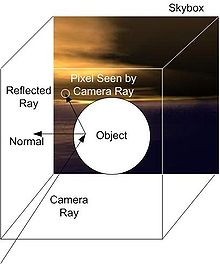
\includegraphics{Cube_mapped_reflection_example}

  \vspace{3mm}
  \parbox{9.5cm}{\caption[Cube mapping visualized.]{A visualization of cube
      mapping. The environment is rendered onto the sides of the cube and then
      mapped onto the object inside the cube map. The mapping is performed by
      using the calculated reflection vector as an index into the cube
      map.\\Image from
      http://en.wikipedia.org/wiki/Reflection\_mapping}\label{fig:cubemap}}
\end{figure}

% Ray tracing and comparing it to rasterization

An alternative to rasterization is \textit{ray tracing}, which elegantly solves
reflection and refraction by tracing rays from the viewer's eye and into the
scene, spawning and tracing new reflection- and refraction rays as needed when
geometry is intersected. A comparisson of cube mapping and ray tracing is given
in \reffig{fig:reflectingDragons}, where I have rendered a reflecting Stanford
Dragon using both techniques. Notice how the ray traced dragons backside
reflects its neck, while the cube mapped version only reflects the surrounding
box. Advanced lighting techniques that produce photorealistic images are also
based on ray tracing. One such technique is \textit{photon mapping}, which can
accurately reproduce the effects of light bouncing of reflective surfaces,
caustics and color bleeding.

\fixme{Write something about how all figures are my own unless explicitly
  stated!}


% High cost used to make it unattractive for interactive scenes

The increased realism that can be achieved by using ray tracing does come at a
high computational cost, which has previously made it unattractive for
interactive applications or dynamic scenes. Nonetheless, the recent increase in
computational power coupled with research into the area of \textit{interactive
  ray tracing} has yielded some remarkable results, and scenes of approximately
100k triangles can now be ray traced in real-time, even with effects such as
shadows, reflection and refraction added.

\begin{figure}
  \centering
  \subfloat[A cube mapped reflecting dragon.]{
    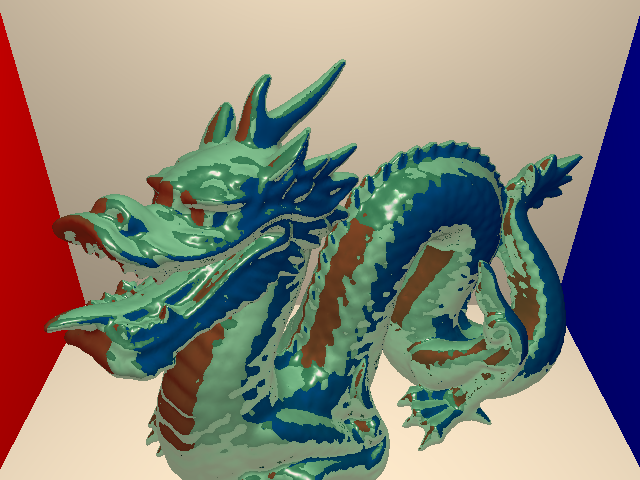
\includegraphics[width=7cm]{cubemappedDragon}
    \label{fig:cubeDragon}
  }
  \hspace{10pt}
  \subfloat[A ray traced reflecting dragon. Notice the self reflection
    on the back and inside the mouth.]{
    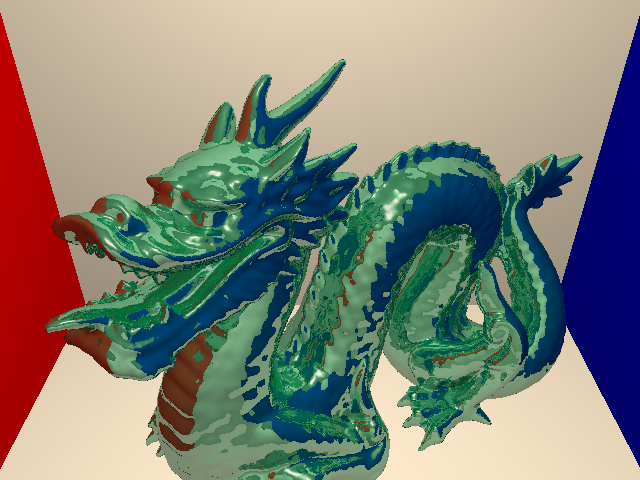
\includegraphics[width=7cm]{semiReflectingDragon}
    \label{fig:rayReflectingDragon}
  }
  \caption[Reflections created with cube mapping and ray tracing.]{An example of
    the difference between using cube mapping or ray tracing for
    reflections.}
  \label{fig:reflectingDragons}
\end{figure}


% What I will show, doing it dynamically, which is interesting for
% games and movie development

With the continued increase in computational power of both CPUs and GPUs, ray
tracing is becoming an increasingly interesting alternative to rasterization. In
this thesis I will examine \textit{ray tracing of dynamic scenes}, with the
express goal to minimize the time between modifying the scene and presenting a
user with visual feedback of the change. This would be very interesting in the
film industry where ray tracers are used to create
\textit{CGI}\footnote{Computer-generated Imagery} effects and the 3D artists
need fast visual feedback while modifying the scene.

%% In this thesis I will examine \textit{ray tracing of dynamic scenes}, which is
%% becoming an interesting alternative to rasterization in the gaming industry in
%% the years to come. The film industry has also used ray tracing to do their
%% \textit{CGI}\footnote{Computer-generated Imagery} effects for quite some time,
%% and for the 3D artists working on these effects, it would certainly be
%% beneficial to use a ray tracer that is able to produce fast visual feedback,
%% when an artist rearranges the scene.

% We need Acceleration stuctures for ray tracing to achieve this

To improve the performance of ray tracers, several acceleration structures have
been developed. The most popular structures are \textit{hierarchical data
  structures}, such as trees, and ray tracers that traverse these are called
\textit{hierarchical ray tracers}. When a ray traverses a hierarchical data
structure it is in search of the nearest leaf node, which contains references to
the geometry nearest to the ray. If the ray finds that it did not see, or
\textit{intersect}, any of the geometry in the current leaf node, it advances
beyond that leaf and performs another traversal of the structure.

The structure employed in this thesis is the \textit{kd-tree}, a binary, space
partitioning tree-structure, which recursively subdivides $k$-dimensional
geometry by splitting it with \textit{axis aligned splitting planes}. Each
interior node in the tree contains a splitting plane and a reference to the
location of its left and right children, while the leafs contain references to
the geometry associated with them. 
%% An example of a subdivided scene and the corrosponding tree can be seen on
%% \reffig{fig:kdIteration} in \refchapter{chp:kdTrees}, where kd-trees will be
%% introduced thoroughly. 
If a leaf node is split by a splitting plane, the geometry associated with that
leaf must be associated with its two newly constructed child nodes. The quality
of a kd-tree is defined as the ease with which it allows a scene to be ray
traced and is affected by the choice of splitting planes. A lot of computational
power can go into finding optimal splitting planes, as there are infinitely many
possible \textit{splitting plane candidates}, or \textit{split candidates}, to
consider.

%% In a high quality kd-tree, splitting planes have been chosen such that
%% spatially close geometry are allocated into the same subtree and the scene
%% can be ray traced as fast as possible. Choosing a splitting plane for a node
%% is the topic of \refsection{sec:splittingPlane}.

In order to facilitate dynamic scenes, the data structure must also be
dynamic. It is possible to dynamically add and remove elements to a kd-tree, but
doing so can degrade the quality of the kd-tree or its subtrees. If a subtree's
quality has degraded too much, it will have to be reconstructed to again
facilitate fast ray tracing. In the worst case scenario this reconstruction
needs to be performed on the entire tree and is equivelant to a complete
reconstruction. Because of this, the algorithms for creating and restructuring
kd-trees needs to be very fast, and might even have to sacrifice tree quality
for improved construction speed. This tradeoff between speed and quality is also
what makes dynamic scenes interesting compared to static scenes. Ray tracers
rendering static scenes can use as much time as needed to produce acceleration
structures of high quality. This may not be possible in dynamic scenes, where a
user that modifies the scene will want visual feedback of the modifications made
as fast as possible.

In general there are three ways to optimize ray tracing with respect to dynamic
scenes to achieve maximum efficiency:

\begin{enumerate}
  \item \textbf{Building a higher quality acceleration structure -} An
    acceleration structure of higher quality will reduce the time it takes the
    ray tracer to find the nearest intersecting point between a ray and the
    scene. Algorithms for producing kd-tree's of different quality is the topic
    of \refsection{sec:splittingPlane}.
  \item \textbf{Build the acceleration structure faster -} As described above,
    the acceleration structure may need to be entirely reconstructed each time a
    dynamic scene is rendered. Being able to rebuild it fast is therefore
    crucial. One way to ensure a faster reconstruction is by reducing the time
    spent deciding where to place the splitting plane, which can result in trees
    of lower quality.
  \item \textbf{Create a faster ray tracer -} Several optimizations exist that
    improve the speed of a ray tracer without modifying the underlying
    acceleration stucture. Such optimizations will be discussed in
    \refsection{sec:hierarchicalTraversal}.
\end{enumerate}


% Why do it on the GPU, yes why indeed? Leaves the CPU free to do
% other things than rendering.

As observed at the beginning of this chapter, GPU's have grown quite powerful
over the last decade, and since the introduction of programmable GPU's and
NVIDIA's \textit{CUDA}\footnote{Compute Unified Device Architecture.}
framework, many algorithms have been succesfully ported to utilize the resources
of the GPU. In this thesis I too will use the massive computational power of the
GPUs to accelerate the creation of data structures and ray tracing them. The
most compelling reason to do this, is that it leaves the CPU free to handle
other aspects of a graphics application, such as game logic and networking
communication.

%% However, the results achieved in this thesis with respect to ray tracing dynamic
%% scenes are architecture independent and apply to the CPU aswell as the GPU.

%% Describe and reference previous work that is relevant to your work.

%% The previous work section is mostly descriptive.

%% Address the weaknesses of the previous methods.

%% You should not do a full comparison between your method and previous
%% work here. Leave that for the Results section.

%% You can however distinguish yourself from previous work by saying
%% something like ”In contrast to method X, my method...”, or ”The main
%% difference between my work and X is...”.

\newpage
\fixme{Make sure this starts on a newline if needed}

\section{Previous Work}

\chapterquote{If you want to make an apple pie from scratch, you must
  first create the universe.}{Carl Sagan}


% Early ray tracing

Arthur Appel\citebook{Appel:1968} is credited as the being the first to describe
the basic idea of ray casting, applying it to solve the \textit{hidden surface
  problem} and to enhance the perception of depth by computing shadows in opaque
polygonal scenes. Whitted\citebook{Whitted:1979} extended the idea of ray
casting into the general recursive ray tracing algorithm still used today. If a
ray would hit a surface, then depending on the surface's material proporties it
could generate any number of new rays, reflection, refraction or shadow.


% Data structures for acceleration

Since then a lot of time and effort has gone into improving the performance of
ray tracing and several data structures have been proposed with this in mind. In
1976 Clark\citebook{Clark:1976:HGM:360349.360354} was the first to suggest using
\textit{bounding volumes} to perform geometry culling and in 1986 Goldsmith and
Salmon\citebook{Goldsmith:1987} extended this idea with an algorithm for
automatically building \textit{bounding volume hierarchies}, \textit{BVH}'s,
topdown. Fujimoto, Tanaka and Iwata\citebook{Fujimoto:1986} introduced the use
of \textit{uniform voxel grids} in 1986. Kaplan\citebook{Kaplan:1985} introduced
the use of kd-trees as a spatial partitioning scheme. To decide where to place
the splitting plane he used the now standard \textit{spatial median splitting}
algorithm. Spatial median splitting places the splitting plane at the middle of
a node's bounding box along some axis, usually either the longest or an axis
chosen in a \textit{round robin} fassion.


% Surface Area Heuristic 

The idea of automatically creating hierarchical acceleration structures have
since been revisited and improved upon countless times. One of the most
important improvements was the introduction of the \textit{Surface Area
  Heuristic}, \textit{SAH}, generally attributed to MacDonald and
Booth\citebook{MacDonald:1990}. SAH estimates the expected cost of ray tracing a
node's two child nodes with respect to some splitting plane. Given a list of
splitting planes, the expected cost for all these planes can then be calculated
and the plane with least cost is chosen as the splitting plane.
%% How exactly this list of splitting planes is created in the first place will be
%% discussed in \refsection{sec:splittingPlane}.


% Havran and kd trees are best?

In his ph.d. thesis\citebook{Havran:PhD} from 2000, Havran argued that the
kd-tree was the best known acceleration structure for ray tracing. While a lot
of new data structures have since appeared, the kd-tree is still one of the most
widely used structures due to its low memory footprint, fast ray/plane
intersection test and countless research papers devoted to both optimal creation
and ray tracing. For these same reasons this thesis will focus on the use of
kd-trees as its acceleration structure.



% GPU acceleration structures

Because of the lack of looping and branching on early programmable graphics
hardware, the first all GPU based ray tracers had to make use of non
hierarchical acceleration structures like grids\citebook{844181}. Grid's,
however, do not scale aswell as hierarchical structures and, in large sparse
scenes, fine-grained grids run the risk of wasting memory on a lot of empty
cells, while more coursely grained grids might store most of the geometry in a
few cells and thus not partition it effectively.

% Traversing the tree and doing it fast

With the addition of branching and looping on graphics hardware, several GPU
based hierarchical ray tracers were proposed. A known optimization to CPU based
hierarchical ray tracers is to use a stack of neighbouring nodes that the ray
could possibly traverse. This is used as a means to prevent restarting ray
tracing from the root of the acceleration structure, if a ray does not intersect
any primitives in its current leaf. Small amounts of available memory per thread
on the graphics card made this optimization technique infeasable for GPU
solutions. Instead Popov et al.\citebook{popov:07:GPURT} in 2007 introduced a
stackless ray tracer rivalling CPU ray tracers in speed, which preprocessed the
kd-tree and adds \textit{ropes}, or references, between neighbouring
nodes. Concurrently \horn{} proposed a different but equally effective
solution. Instead of storing the entire stack of possible neighbouring nodes, a
\textit{short-stack} of only the $N$ lowest possible nodes was stored in
memory. Horn et al. also introduced an optimization called \textit{push-down},
where each ray did not restart at the root of the tree, but instead at the root
of the smallest subtree enclosing the ray. Finally they showed how this could be
implemented together with \textit{packet tracing}, where several rays are traced
in packets by one thread to amortize the cost of traversing the tree.

%% In this thesis I've adopted Horn et al.'s idea of a short stack to
%% improve our ray tracer. In a worst case scenario where all the rays
%% are intersecting the root node's splitting plane, the push-down approch
%% yields no improvement, but only adds a computational overhead, which
%% can also be seen in the papers results section. Therefore I have
%% chosen not to implement it. With the increased detail in ray traced
%% scenes, ray directions may become more and more chaotic after the
%% primary rays have been cast. Due to this, packet tracing may not be
%% one of the best long term optimizations. In this thesis I will instead
%% show how grouping spatially close primary rays into clusters will
%% drastically improve ray tracing efficiency, with hardly any added
%% extra logic.


% Previously constructing the KD-tree was most effective on the CPU,
% optimized and fast for multi core CPU's

Although ray tracing on graphics hardware had been made as fast as its CPU
counterparts by 2007, creating kd-trees on the GPU had still not been done
efficiently.

% Recent research has made it possible to construct KD-trees
% efficiently on GPU's

This changed in 2008 when \zhou{} introduced \textit{breath-first} tree creation
on the GPU. Instead of creating kd-trees in \textit{depth-first} manner, in
which only one node was processed at a time, their breath-first algorithm made
it possible to work on hundreds or thousands of nodes in parallel, allowing it
to scale much better with the architecture of graphics cards. For the uppermost
nodes in the tree they proposed to parallelize the calculation of the node split
cost across all geometric primitives, creating thousands of threads. For the
lower part of the tree, where thousands of nodes needed to calculate their split
cost, computations were simply parallelized over all available nodes.


% KD-tree work and what we've made differently

%% The kd-tree construction work done in this thesis is greatly inspired
%% by Zhou et al.\citebook{1409079}. My approch to upper tree nodes is
%% nearly identical to theirs; using spatial median splitting for
%% determining where to place the splitting plane and optimizing the tree
%% by maximizing empty space. I will however also be focusing on how to
%% handle triangles cut by the splitting plane and discuss 2 alternatives
%% to a standard splitting approach. In the case of lower nodes I will
%% compare the computation intensive SAH, as used by \zhou, to 2 other
%% methods. The first trivially stops tree creation at the upper trees
%% leafs, while the second method will create balanced subtrees.


\section{Goals}

In this thesis the goal is not to produce images of photorealistic quality, or
create an interactive ray tracer \footnote{This goal alone can be achieved
  trivially by reducing the complexity of the ray traced scene or lowering the
  image resolution.}. Instead this thesis will explorer ray tracing acceleration
structures, specifically the kd-tree, and its impact on ray tracing efficiency
for dynamic scenes.

The main topic in this thesis is the relationship between the time spend
constructing a kd-tree and its resulting quality, i.e. how fast can it
accelerate ray tracing. Building on the kd-tree implementation presented by
\zhou{}, I will investigate different parts of the kd-tree construction phase
for dynamic scenes and whether it is worthwile in dynamic scenes to sacrifice
tree quality to gain faster kd-tree construction. The two parts of the kd-tree
creation phase that will be investigated is the choice of splitting plane and
how geometry is associated with child nodes after a split. As part of this
investigation I will describe several different solutions and show how to
implement them efficiently on dataparallel GPUs using CUDA.

The kd-trees created by the different methods above will be evaluated by how
fast they can be constructed and how efficiently a ray tracer can traverse them
to render a scene. During evaluation I will always perform a complete rebuild of
the kd-tree before rendering a scene. This is done to ensure that my tests
capture the worst case scenario for dynamic scenes, which is a complete update
of the entire scene and thus a complete rebuild. The goal of this thesis is then
to find a kd-tree configuration that minimizes the total time spent both
recreating and traversing the acceleration structure and evaluate the tradeoff
between construction speed and tree quality.

I will furthermore discuss the ray tracers used to evaluate the quality of the
kd-trees. To provide a fair and useful comparison of a kd-tree's construction
time and its quality, I will need to create a highly optimized ray tracer. These
optimizations are important as a fully optimized ray tracer can render scenes up
to 70\% faster than a basic implementation and does so independent of the
underlying kd-tree and its construction schemes. While I will be discussing and
applying these optimizations, such as the short-stack optimization from \horn{},
the topic is secondary to kd-trees and merely included for evaluation purposes.

Given the added overhead of continuously rebuilding the kd-trees, an interesting
question is whether or not we even need them. I therefore present an
\textit{exhaustive ray tracer}, which does not use any acceleration structure
and thus intersects every ray with every triangle. The exhaustive ray tracer
will be compared to the hierarchical ray tracers and hopefully motivate the
continued use of acceleration structures for dynamic scenes.

\section{Overview}

The rest of the thesis is structured as follows:

% Previous work

%% The next section details previous work in the area of ray tracing and
%% kd-tree construction. This includes a brief history of when ray
%% tracing was introduced, aswell as key points in time for different
%% acceleration structures. The last part of this section will focus on
%% kd-trees and ray tracing on graphics hardware. Changes in this thesis
%% compared to previous work in the area are also outlined in this
%% section.

% Understanding CUDA

\refchapter{chp:GPGPU} introduces NVIDIA's CUDA framework. Here I will describe
its thread and memory model. I will then go on to describe a new primitive
proposed by \sengupta{}, which will be needed, e.g. when assigning triangles to
child nodes after their parent node has been split. The last part of this
chapter will focus on optimization techniques specific to CUDA and apply these
incrementally in a case study of a global minima algorithm.

% kd-trees

\refchapter{chp:kdTrees} is devoted to discussing the construction of
kd-trees. The first part of this section deals with the general kd-tree
construction algorithm. Here I will present several algorithms for choosing the
splitting plane and discuss three different approaches used to associate
triangles with leaf nodes. The second part of \refchapter{chp:kdTrees} deals
with the actual implementation of kd-trees on a GPU and will describe how the
nodes are structured in memory and how to construct binary trees effectively on
dataparallel hardware.

% ray tracing

Having introduced kd-trees, \refchapter{chp:rayTracing} will deal with the
algorithms for traversing such trees and ray tracing a scene. Here several
optimizations to a basic hierarchical ray tracer will be discussed and
incrementally added. First though, an exhaustive ray tracer is presented and
will be used in teh Conclussion to motivate the use of hierarchical data
structures. This chapter also includes a discussion of two triangle intersection
algorithms with respect to achieving maximal performance on GPUs.

% Results

In \refchapter{chp:results} I will first evaluate the performance of several
different ray tracers. I will then use the ray tracer that generally performs
best to evaluate the quality of the different kd-trees created. The metric used
to determine which kd-tree construction algorithm performs best will be the
total rendering time, i.e. the sum of the construction time and ray tracing
time.

% Conclusion % Future work

I will then conclude my work by discussing my results and their implications for
the future of ray tracing dynamic scenes. Finally in \refchapter{chp:future} I
will address future improvements based on the experience I have gained while
working on this thesis.

